\documentclass[12pt, a4paper]{article}

\usepackage{polski}
\usepackage[utf8]{inputenc}
\usepackage[T1]{fontenc}
\usepackage{geometry}
\usepackage{graphicx}
\usepackage{fancyhdr}
\usepackage{amsmath}
\usepackage{caption}
\usepackage{subcaption}
\usepackage{tikz}
\usepackage{amsfonts}
\usepackage{listings}
\usepackage{textcomp}

\newgeometry{tmargin=2cm, bmargin=2cm, lmargin=2cm, rmargin=2cm}

\setlength{\parindent}{10mm}
\setlength{\parskip}{4mm}

\definecolor{listinggray}{gray}{0.9}
\definecolor{lbcolor}{rgb}{0.9,0.9,0.9}
\lstset{
backgroundcolor=\color{lbcolor},
    tabsize=4,    
%   rulecolor=,
    language=[GNU]C++,
        basicstyle=\scriptsize,
        upquote=true,
        aboveskip={1.5\baselineskip},
        columns=fixed,
        showstringspaces=false,
        extendedchars=false,
        breaklines=true,
        prebreak = \raisebox{0ex}[0ex][0ex]{\ensuremath{\hookleftarrow}},
        frame=single,
        numbers=left,
        showtabs=false,
        showspaces=false,
        showstringspaces=false,
        identifierstyle=\ttfamily,
        keywordstyle=\color[rgb]{0,0,1},
        commentstyle=\color[rgb]{0.026,0.112,0.095},
        stringstyle=\color[rgb]{0.627,0.126,0.941},
        numberstyle=\color[rgb]{0.205, 0.142, 0.73}
}
\lstset{
    backgroundcolor=\color{lbcolor},
    tabsize=4,
  language=C++,
  captionpos=b,
  tabsize=3,
  frame=lines,
  numbers=left,
  numberstyle=\tiny,
  numbersep=5pt,
  breaklines=true,
  showstringspaces=false,
  basicstyle=\footnotesize,
%  identifierstyle=\color{magenta},
  keywordstyle=\color[rgb]{0,0,1},
  commentstyle=\color{Darkgreen},
  stringstyle=\color{red}
  }

\includeonly{symulator}
 
\begin{document}
    
    \pagestyle{fancy}
    \renewcommand{\headrulewidth}{0pt}
    \renewcommand{\footrulewidth}{0.4pt}
    \fancyhead{}
    \lfoot{\textit{WSSiS SCADA --~semestr zimowy 2016/2017}}
    \cfoot{}
    \rfoot{\textit{Strona \thepage}}
    
    \begin{titlepage}
        \title{
        \centering
        
\includegraphics[width=3cm]{../img/agh_logo.jpg}\\[1cm]
        \textit{\Large{Akademia Górniczo-Hutnicza im. Stanisława Staszica\\ w
        Krakowie}}\\[0.7cm]
        \large{\textsc{Wielopoziomowe struktury sterowania i~systemy
        SCADA}}\\[1cm]
        \rule{\textwidth}{1.6pt}\vspace*{-\baselineskip}\vspace*{2pt}
        \rule{\textwidth}{0.4pt}\\[\baselineskip]
        \Huge{\textsc{Model układu chłodzenia cieczą wraz z~panelem
        operatorskim wykonanym z~wykorzystaniem biblioteki graficznej Qt}}
        \rule{\textwidth}{0.4pt}\vspace*{-\baselineskip}\vspace{3.2pt}
        \rule{\textwidth}{1.6pt}\\[\baselineskip]}
        \author{\textit{Autorzy:}\\
        \Large{Adasiewicz Konrad} \\
        \Large{Maciejewski Michał}}
        \date{\textit{Data wykonania:}\\ \today}
        \maketitle
        \thispagestyle{empty}
    \end{titlepage}

    \tableofcontents

    \section{Wstęp}
\indent

Celem projektu przedstawionego w~poniższym sprawozdaniu było stworzenie modelu
układu chłodzenia cieczą oraz oprogramowania do nadzorowania tego procesu
--~systemu SCADA. W~ramach zrealizowanych dotychczas zajęć możliwe było
zapoznanie się z~profesjonalnymi narzędziami służącymi do kontrolowania
przebiegu procesu na przykładzie oprogramowania \textit{zenon}.

Posiadając już doświadczenie w~obsłudze dedykowanych rozwiązań, które mimo
swojego zaawansowania sprawiają niekiedy wrażenie, czasami aż nadmiernie,
skomplikowanych i~topornych, nadrzędnym zadaniem stała się próba wykonania
panelu operatorskiego z~wykorzystaniem narzędzi typowo programistycznych, czyli
języka \textit{C++} oraz biblioteki graficznej \textit{Qt}. Możliwość
samodzielnego wpływania na budowę i~złożoność tworzonego oprogramowania oraz
wszystkie jego funkcjonalności była bardzo zachęcającym argumentem przy
podejmowaniu wyboru odnośnie tematu poniższej pracy. W~związku z~tym, w~wielu
miejscach będą pojawiały się porównania do pakietu \textit{zenon}, głównie
dotyczące aspektów obsługi.

Dodatkowym elementem prac było wykorzystanie płytki ewaluacyjnej firmy
\textit{STMicroelectronics} do symulowania sterownika modelowanego układu.
Również w~tym miejscu pojawił się pomysł przetestowania alternatywnych,
relatywnie prostszych w~porównaniu do przemysłowych, protokołów komunikacyjnych
pomiędzy komputerem a sterownikiem.

Najważniejszym czynnikiem decydującym o~powodzeniu projektu była poprawność
działania oraz stabilność stworzonego oprogramowania, co również zostało
przetestowane i~opisane w~odpowiednich rozdziałach poniższego sprawozdania.

    \section{Model matematyczny}
\indent

W~poniższym rozdziale przedstawiona została konstrukcja modelu matematycznego
układu chłodzenia cieczą procesora komputera oraz wyznaczanie odpowiednich
parametrów tego modelu.

Na podstawie informacji znalezionych na stronie \cite{EKWBsite} oraz na forach
zajmujących się tematyką chłodzenia wodnego komputera, możliwe było
zaprojektowanie prostej pętli, w~skład której wchodził blok wodny, którego
zadanie polegało na odbieraniu ciepła z~powierzchni procesora oraz radiator
(chłodnica) oddający ciepło do otoczenia. Dodatkowym niezbędnym elementem była
pompa wymuszająca obieg wody w~układzie oraz wentylatory umieszczone na
radiatorze wspomagające przepływ powietrza.

Równania różniczkowe opisujące powyższe elementy układu chłodzenia przedstawione
są w~kolejnych podrozdziałach. Do ich konstrukcji (w~przypadku opisu przepływu
ciepła) zastosowane zostało prawo Fouriera przy pewnych założeniach:
\begin{itemize}
    \item materiały, z~których wykonany jest blok wodny oraz chłodnica są
    jednorodne,
    \item w~związku z~powyższym, przepływ ciepła przez te materiały również jest
    jednorodny,
    \item matematyczny opis wymiany ciepła jest uproszczony.
\end{itemize}

\subsection{Równania pompy i~wentylatorów}
\indent

Pompa wody oraz wentylatory w~układach chłodzenia cieczą są zwykle zasilane
z~jednego z~napięć dostarczanych przez zasilacz komputera --~$5$ lub $12$~[$V$],
w~zależności od producenta. Rodzaj wykorzystanych silników oraz sposób
sterowania nimi nie był jednak tematem tej pracy, przez co przyjęte zostały
pewne uproszczenia odnośnie sterowania --~pomijany jest dokładny sposób
zasilania oraz opis matematyczny. Założenie polegało na przyjęciu, iż zarówno
zachowanie silnika pompy jak i~wentylatorów można z~pewnym przybliżeniem
przedstawić w~postaci równania różniczkowego pierwszego rzędu --~jako inercję
pierwszego rzędu. Wartości sterowań określały natomiast współczynnik
wypełnienia dla sygnałów PWM wykorzystywanych w~układach zasilania silników.

Wentylatory umieszczone na chłodnicy wykorzystywały wspólny sygnał zasilający,
przez co można je było traktować w~uproszczeniu jako jeden większy wentylator
o~odpowiednio dobranych parametrach. W~związku z~tym, do układu doprowadzane
były dwa sygnały sterujące:
\begin{itemize}
    \item $u_1$ --~sygnał sterujący pompą wody,
    \item $u_2$ --~sygnał sterujący wentylatorami,
\end{itemize}
gdzie $u_i \in \left[ 0; 1 \right]$, $i = 1, 2$.

Modele przyjęte dla pompy oraz wentylatorów były inercjami pierwszego rzędu,
a~zatem --~dobierając odpowiednie wzmocnienia --~równania różniczkowe opisujące
te obiekty przedstawiały się następująco:
\begin{equation}
    \dot{x_1} = k_w \cdot \left( u_1 - x_1 \right)
    \label{equ:x1}
\end{equation}
\begin{equation}
    \dot{x_2} = k_a \cdot \left( u_2 - x_2 \right)
    \label{equ:x2}
\end{equation}
gdzie:
\begin{itemize}
    \item $x_1$ --~prędkość obrotowa pompy wody,
    \item $x_2$ --~prędkość obrotowa wentylatorów,
    \item $k_w = 2$ --~współczynnik wzmocnienia dla pompy,
    \item $k_a = 1.25$ --~współczynnik wzmocnienia dla wentylatorów.
\end{itemize}

Wartości prędkości obrotowych, zarówno pompy jak i~wentylatorów, zawierały się
w~przedziale $x_i \in \left[ 0; 1 \right]$, $i = 1, 2$, co wynika wprost
z~równań \eqref{equ:x1} oraz \eqref{equ:x2}. Odpowiednie współczynniki
skalujące wpływające na przepływ wody lub powietrza zostały pobrane ze
specyfikacji przykładowej pompy \cite{EKWBpump} oraz wentylatora \cite{EKWBfan}
i~umieszczone w~równaniach, które wykorzystują te przepływy --~wartości $F_i
\text{,} \quad i \in \left\{ w, a \right\}$ w~równaniu \eqref{equ:x4} oraz
\eqref{equ:x5}. Natomiast współczynniki wzmocnienia dla pompy i~wentylatorów
zostały dobrane jedynie w~taki sposób, aby zróżnicować zachowanie tych elementów
układu.

\subsection{Równanie temperatury struktury krzemowej procesora}
\indent

W~celu wyznacznia równania opisującego przepływ ciepła przez blok wodny
wykorzystane zostało pojęcie rezystancji termicznej \cite{ThermalResistance}.
Opisana jest ona równaniem:
\begin{equation}
    R_{th} = \frac{\Delta T}{Q}
    \label{equ:thermalresistance}
\end{equation}
gdzie:
\begin{itemize}
    \item $R_{th}$ --~rezystancja termiczna materiału,
    \item $\Delta T$ --~różnica temperatur między powierzchniami materiału,
    \item $Q$ --~ilość energii cieplnej przepływającej przez materiał
    w~jednostce czasu (moc cieplna).
\end{itemize}

Rezystancja termiczna jest zwykle bardzo trudna do wyznaczenia, gdyż zależy od
wielu czynników. W~przypadku prostych elementów lub układów elektronicznych,
takich jak diody wysokoprądowe, tranzystory, wzmacniacze scalone i~inne, jest
ona podawana w~notach katalogowych tych elementów. Niestety znalezienie tego
parametru dla obudowy procesora komputerowego i~bloku wodnego nie należy już do
tak prostych, gdyż producenci nie umieszczają takich informacji w~dostępnych
publicznie broszurach.

W~takiej sytuacji, rezystancja bloku wodnego oraz obudowy procesora (jako
całości) została wyznaczona korzystając z~tego, że takie układy w~rzeczywistości
istnieją i~funkcjonują prawidłowo. Typowa maksymalna wartość mocy cieplnej
wydzielanej przez procesor dla najbardziej wydajnych konstrukcji wynosi
$Q_{max} = 140$~[$W$] --~jako przykład został wykorzystany procesor
\textit{Intel i7-5960X} \cite{Inteli7}. Maksymalna dopuszczalna temperatura
złącza krzemowego wynosi zwykle $T_{CPU_{max}} = 100$~[$^\circ C$]. Maksymalna
temperatura wody w~układzie chłodzenia jest uzależniona od konstrukcji pompy
i~jej odporności. Na przykładzie pompy \textit{EK-D5 PWM G2 Motor}, której
specyfikacja znajduje się na stronie \cite{EKWBpump}, wartość tej temperatury
wynosi $T_{w_{max}} = 60$~[$^\circ C$]. Przy założeniu stałej temperatury
struktury krzemowej procesora, cała energia cieplna jest transportowana przez
obudowę i~blok do wody, tak więc rezystancja termiczna wynosi:
\begin{equation}
    R_{th} = \frac{T_{CPU_{max}} - T_{w_{max}}}{Q_{max}} = \frac{100 - 60}{140}
    \left[ \frac{^\circ C}{W} \right] \approx 0.3 \left[ \frac{^\circ C}{W}
    \right]
    \label{equ:wbresistance}
\end{equation}

W~przypadku braku równowagi termodynamicznej, czyli gdy ilość energii
wydzielanej w~strukturze procesora jest różna od odbieranej przez wodę,
następuje zmiana temperatury struktury krzemowej. Opisywana jest ona następującą
zależnością:
\begin{equation}
    K_1 \cdot \Delta T_{CPU} = Q_{IN} - \frac{T_{CPU} - T_c}{R_{th}}
    \label{equ:dtcpu}
\end{equation}
gdzie:
\begin{itemize}
    \item $K_1$ --~współczynnik zmian temperatury struktury krzemowej procesora,
    \item $\Delta T_{CPU}$ --~przyrost temperatury struktury krzemowej
    w~jednostce czasu,
    \item $T_{CPU}$ --~aktualna temperatura struktury krzemowej procesora,
    \item $T_c$ --~aktualna temperatura wody wypływającej z~bloku wodnego (wody
    ciepłej).
\end{itemize}

Współczynnik zmian temperatury struktury krzemowej jest zależny od dwóch
czynników --~masy tej struktury oraz jej ciepła właściwego. Wartości te wynoszą
odpowiednio:
\begin{itemize}
    \item $m_{CPU} = 0.01$~[$kg$],
    \item $c_{CPU} = 710$~[$\frac{J}{kg \cdot K}$]
\end{itemize}
Masa struktury została przyjęta na podstawie średnich wartości wag procesorów,
które zostały znalezione w~różnych źródłach internetowych (przy pominięciu masy
laminatu i~obudowy). Natomiast ciepło właściwe struktury jest równe ciepłu
właściwemu krzemu. Zmieniając oznaczenia zmiennych uzyskano następującą
zależność, która jest równaniem różniczkowym opisującym zmiany temperatury
struktury krzemowej procesora:
\begin{equation}
    \dot{x_3} = \frac{Q_{IN}}{m_{CPU} \cdot c_{CPU}} - \frac{x_3 - x_4}{m_{CPU}
    \cdot c_{CPU} \cdot R_{th}}
    \label{equ:x3}
\end{equation}
gdzie:
\begin{itemize}
    \item $x_3$ --~temperatura struktury krzemowej,
    \item $x_4$ --~temperatura wody wypływającej z~bloku wodnego (wody ciepłej).
\end{itemize}

\newpage

\subsection{Równanie wody ciepłej}
\indent

Woda ciepła w~układzie chłodzenia to woda wypływająca z~bloku wodnego
i~płynąca z~niego do chłodnicy. W~stanie ustalonym ilość energii cieplnej
przekazywanej w~jednostce czasu przez blok wodny ze struktury procesorowej jest
równa energii odbieranej przez wodę w~tym bloku:
\begin{equation}
    \frac{T_{CPU} - T_c}{R_{th}} = K_2 \cdot \left( T_c - T_z \right)
    \label{equ:hotwater}
\end{equation}
gdzie:
\begin{itemize}
    \item $K_2$ --~współczynnik odbierania ciepła przez wodę w~bloku wodnym,
    \item $T_z$ --~temperatura wody wpływającej do bloku wodnego (wody zimnej).
\end{itemize}

Wartość współczynnika $K_2$ zależna jest od ciepła właściwego wody oraz masy
wody przepływającej przez blok wodny w~jednostce czasu:
\begin{equation}
    K_2 = m_{wb} \cdot c_w
    \label{equ:k2}
\end{equation}
Ilość wody przepływającej przez blok wodny jest zależna od aktualnej prędkości
obrotowej pompy wody --~na podstawie równania \eqref{equ:x1} --~oraz jej
wydajności:
\begin{equation}
    m_{wb} = x_1 \cdot m_{wb_{max}}
    \label{equ:mwb}
\end{equation}
W~specyfikacji przykładowej pompy \cite{EKWBpump} producent informuje, iż jej
wydajność wynosi $F_w = 1500$~[$\frac{l}{h}$], czyli $F_w =
\frac{1.5}{3600}$~[$\frac{m^3}{s}$], natomiast gęstość wody jest równa $\rho_w
= 1000$~[$\frac{kg}{m^3}$], co prowadzi do zależności:
\begin{equation}
    m_{wb_{max}} = F_w \cdot \rho_w
    \label{equ:mwbmax}
\end{equation}

Podstawiając powyższe do równania \eqref{equ:hotwater} otrzymano następującą
zależność, która obowiązuje w~stanie ustalonym --~przy ilość energii oddawanej
w~jednostce czasu przez procesor równej ilości odbieranej przez wodę:
\begin{equation}
    \frac{T_{CPU} - T_c}{R_{th}} = x_1 \cdot F_w \cdot \rho_w \cdot c_w \cdot
    \left( T_c - T_z \right)
    \label{equ:hotwaterfull}
\end{equation}
W~sytuacji, gdy układ ten nie znajduje się w~równowadze termodynamicznej
następuje zmiana temperatury wody ciepłej, która opisana jest poniższym
równaniem:
\begin{equation}
    K_3 \cdot \Delta T_c = \frac{T_{CPU} - T_c}{R_{th}} - x_1 \cdot F_w \cdot
    \rho_w \cdot c_w \cdot \left( T_c - T_z \right)
    \label{equ:dtc}
\end{equation}
gdzie:
\begin{itemize}
    \item $K_3$ --~współczynnik zmian temperatury wody ciepłej,
    \item $\Delta T_c$ --~przyrost temperatury wody ciepłej w~jednostce czasu.
\end{itemize}

Wartość współczynnika $K_3$ jest zależna od masy wody w~bloku wodnym oraz
ciepła właściwego wody:
\begin{itemize}
    \item $m_b = 0.15$~[$kg$],
    \item $c_b = 4190$~[$\frac{J}{kg \cdot K}$].
\end{itemize}
Masa wody została przyjęta na podstawie uśrednionych wartości znalezionych na
stronach producentów i~forach. Przyjmując odpowiednie oznaczenia otrzymano
następującą zależność, która jest równaniem różniczkowym opisującym zmiany
temperatury wody wypływającej z~bloku wodnego --~wody ciepłej:
\begin{equation}
    \dot{x_4} = \frac{x_3 - x_4}{m_b \cdot c_b \cdot R_{th}} - x_1 \cdot F_w
    \cdot \rho_w \cdot c_w \frac{x_4 - x_5}{m_b \cdot c_b}
    \label{equ:x4}
\end{equation}

\subsection{Równanie wody zimnej}
\indent

Woda zimna w~układzie chłodzenia to woda, która wypływa z~chłodnicy i~płynie
z~niej do bloku wodnego. W~stanie ustalonym ilość energii cieplnej
transportowana przez wodę ciepłą w~jednostce czasu jest równa ilości energii
rozpraszanej do otoczenia przez radiator:
\begin{equation}
    x_1 \cdot F_w \cdot \rho_w \cdot c_w \cdot \left( T_c - T_z \right) = K_4
    \cdot \left( T_z - T_o \right)
    \label{equ:coldwater}
\end{equation}
gdzie:
\begin{itemize}
    \item $K_4$ --~wpółczynnik odbierania ciepła przez radiator,
    \item $T_o$ --~temperatura otoczenia.
\end{itemize}

W~przypadku radiatora wartość współczynnika $K_4$ jest sumą dwóch wartości:
\begin{itemize}
    \item $K_{41}$ --~współczynnik swobodnego przepływu powietrza,
    \item $K_{42}$ --~współczynnik wymuszonego przepływu powietrza.
\end{itemize}

Wartość współczynnika $K_{41}$ wynika z~naturalnego zjawiska jakim jest
konwekcja. Zgodnie z~informacjami zawartymi na stronie \cite{CHT} wynosi on:
\begin{equation}
    K_{41} = h_a \cdot A_r
    \label{equ:k41}
\end{equation}
gdzie:
\begin{itemize}
    \item $h_a$ --~współczynnik przenikania ciepła,
    \item $A_r$ --~efektywna powierzchnia radiatora.
\end{itemize}
Wartość współczynnika $h_a$ dla swobodnego przepływu ciepła, według informacji
zawartych na stronie \cite{CHT}, powinna wynosić w~najmniej korzystnym przypadku
$h_a = 0.5$~[$\frac{W}{m^2 \cdot K}$]. Na potrzeby tego układu została ona
jednak jeszcze bardziej zmniejszona z~powodu budowy chłodnicy oraz umieszczenia
na niej wentylatorów, a~co za tym idzie, utrudnień w~swobodnym przepływie
powietrza. Ostatecznie przyjęta została wartość $h_a = 0.1$~[$\frac{W}{m^2
\cdot K}$].

W~przypadku tworzonego układu wybrana została chłodnica o~parametrach
identycznych jak fizycznie dostępny produkt \cite{EKWBradiator}:
\begin{itemize}
    \item $l = 0.52$~[$m$] --~długość,
    \item $w = 0.13$~[$m$] --~szerokość,
    \item $h = 0.038$~[$m$] --~wysokość,
    \item $FPI = 19$~[$\frac{1}{in}$] --~liczba finów (żeberek) na cal.
\end{itemize}
Powierzchnia efektywna chłodnicy zależy nie tylko od jej fizycznych wymiarów,
ale w~dużej mierze od parametru $FPI$. Wpływ wartości tego parametru na budowę
chłodnicy przedstawiony jest na rysunku~\ref{fig:fpicomp}, gdzie widoczny jest
fragment chłodnicy --~widok ,,od przodu''.
\begin{figure}[ht]
    \centering
    \begin{subfigure}{.45\textwidth}
        \centering
        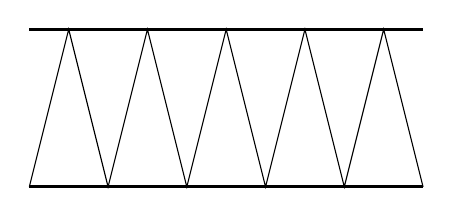
\begin{tikzpicture}
            \draw[very thick] (0, 1) -- (5, 1);
            \draw[very thick] (0, -1) -- (5, -1);
            \draw (0, -1) -- ++(.5, 2) -- ++(.5, -2) -- ++(.5, 2) -- ++(.5, -2)
            -- ++(.5, 2) -- ++(.5, -2) -- ++(.5, 2) -- ++(.5, -2) -- ++(.5, 2)
            -- ++(.5, -2);
        \end{tikzpicture}
        \caption{$FPI = FPI_a$}
    \end{subfigure}
    \begin{subfigure}{.45\textwidth}
        \centering
        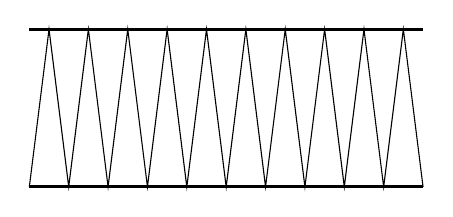
\begin{tikzpicture}
            \draw[very thick] (0, 1) -- (5, 1);
            \draw[very thick] (0, -1) -- (5, -1);
            \draw (0, -1) -- ++(.25, 2) -- ++(.25, -2) -- ++(.25, 2) -- ++(.25,
            -2) -- ++(.25, 2) -- ++(.25, -2) -- ++(.25, 2) -- ++(.25, -2) --
            ++(.25, 2) -- ++(.25, -2) -- ++(.25, 2) -- ++(.25, -2) -- ++(.25, 2)
            -- ++(.25, -2) -- ++(.25, 2) -- ++(.25, -2) -- ++(.25, 2) -- ++(.25,
            -2) -- ++(.25, 2) -- ++(.25, -2);
        \end{tikzpicture}
        \caption{$FPI = FPI_b$}
    \end{subfigure}
    \caption{Porównanie wpływu współczynnika $FPI$ na budowę i~efektywną
    powierzchnię chłodnicy --~$FPI_a < FPI_b$}
    \label{fig:fpicomp}
\end{figure}

Wiedząc w~jaki sposób współczynnik $FPI$ wpływa na efektywną powierzchnię
chłodnicy, możliwe było wyznaczenie jej wartości:
\begin{equation}
    A_r = 2 \cdot \left\lfloor l \cdot \frac{FPI}{0.025} \right\rfloor \cdot w
    \cdot h
    \label{equ:radA}
\end{equation}
Mnożenie przez $2$ w~powyższym wzorze wynika z~tego, że finy mają dwie
powierzchnie, dzielenie przez $0.025$ spowodowane jest koniecznością
przeliczenia wartości współczynnika $FPI$ na jednostki metryczne, natomiast
wyznaczanie podłogi było podyktowane koniecznością otrzymania całkowitej liczby
żeberek w~chłodnicy.

Wartość współczynnika $K_{42}$ wynika z~wymuszonego przepływu powietrza
spowodowanego działaniem wentylatorów i~jej wyznaczanie jest analogiczne jak
w~przypadku współczynnika $K_2$ w~równaniu \eqref{equ:k2}:
\begin{equation}
    K_{42} = m_{ar} \cdot c_a
    \label{equ:k42}
\end{equation}
Ilość powietrza przepływającego przez radiator jest zależna od aktualnej
prędkości obrotowej wentylatorów --~na podstawie równania \eqref{equ:x2} --~oraz
ich wydajności:
\begin{equation}
    m_{ar} = x_2 \cdot m_{ar_{max}}
    \label{equ:mar}
\end{equation}
W~specyfikacji przykładowego wentylatora \cite{EKWBfan} producent informuje, że
jego wydajność wynosi $F_a = 181$~[$\frac{m^3}{h}$], czyli $F_a =
\frac{181}{3600}$~[$\frac{m^3}{s}$], natomiast gęstość powietrza równa jest
$\rho_a = 1.2$~[$\frac{kg}{m^3}$]. Wiedząc, że do wybranej chłodnicy można
przymocować cztery wentylatory, ostatecznie wydajność została ustalona na
wartość $F_a = \frac{4 \cdot 181}{3600}$~[$\frac{m^3}{h}$], co prowadzi do
zależności:
\begin{equation}
    m_{ar_{max}} = F_a \cdot \rho_a
    \label{equ:marmax}
\end{equation}

Podstawiając powyższe do równiania \eqref{equ:coldwater} otrzymano następującą
zależność, która obowiązuje w~stanie ustalonym --~przy ilości energii
transportowanej przez wodę ciepłą w~jednostce czasu równą ilości energii
oddawanej przez radiator do otoczenia:
\begin{equation}
    x_1 \cdot F_w \cdot \rho_w \cdot c_w \cdot \left( T_c - T_z \right) = \left(
    h_a \cdot A_r + x_2 \cdot F_a \cdot \rho_a \cdot c_a \right) \cdot \left(
    T_z - T_o \right)
    \label{equ:coldwaterfull}
\end{equation}
W~sytuacji, gdy układ ten nie znajduje się w~równowadze termodynamicznej
następuje zmiana temperatury wody zimnej, która opisana jest poniższym
równaniem:
\begin{equation}
    K_5 \cdot \Delta T_z = x_1 \cdot F_w \cdot \rho_w \cdot c_w \cdot \left( T_c
    - T_z \right) - \left( h_a \cdot A_r + x_2 \cdot F_a \cdot \rho_a \cdot c_a
    \right) \cdot \left( T_z - T_o \right)
    \label{equ:dtz}
\end{equation}
gdzie:
\begin{itemize}
    \item $K_5$ --~współczynnik zmian temperatury wody zimnej,
    \item $\Delta T_z$ --~przyrost temperatury wody zimnej w~jednostce czasu.
\end{itemize}

Wartość współczynnika $K_5$ jest zależna od masy wody w~chłodnicy oraz jej
ciepła właściwego:
\begin{itemize}
    \item $m_r = 0.235$~[$kg$],
    \item $c_r = 4190$~[$\frac{J}{kg \cdot K}$].
\end{itemize}
Masa wody została przyjęta na podstawie pojemności chłodnicy zawartej
w~specyfikacji umieszczonej na stronie \cite{EKWBradiator}. Przyjmując
odpowiednie oznaczenia otrzymano następującą zależność, która jest równaniem
różniczkowym opisującym zmiany temperatury wody wypływającej z~chłodnicy --~wody
zimnej:
\begin{equation}
    \dot{x_5} = x_1 \cdot F_w \cdot \rho_w \cdot c_w \frac{x_4 - x_5}{m_r \cdot
    c_r} - \left( h_a \cdot A_r + x_2 \cdot F_a \cdot \rho_a \cdot c_a \right)
    \frac{x_5 - T_o}{m_r \cdot c_r}
    \label{equ:x5}
\end{equation}

\subsection{Model układu}
\indent

Model układu chłodzenia cieczą procesora komputerowego dany jest równaniami
\eqref{equ:x1}, \eqref{equ:x2}, \eqref{equ:x3}, \eqref{equ:x4} oraz
\eqref{equ:x5} i~przedstawia się następująco:
\begin{equation}
    f\left( x\left( t \right), u\left( t \right) \right) =
    \begin{cases}
        k_w \cdot \left( u_1 - x_1 \right)\\
        k_a \cdot \left( u_2 - x_2 \right)\\
        \frac{Q_{IN}}{m_{CPU} \cdot c_{CPU}} - \frac{x_3 - x_4}{m_{CPU} \cdot
        c_{CPU} \cdot R_{th}}\\
        \frac{x_3 - x_4}{m_b \cdot c_b \cdot R_{th}} - x_1 \cdot F_w \cdot
        \rho_w \cdot c_w \frac{x_4 - x_5}{m_b \cdot c_b}\\
        x_1 \cdot F_w \cdot \rho_w \cdot c_w \frac{x_4 - x_5}{m_r \cdot c_r} -
        \left( h_a \cdot A_r + x_2 \cdot F_a \cdot \rho_a \cdot c_a \right)
        \frac{x_5 - T_o}{m_r \cdot c_r}
    \end{cases}
    \label{equ:model}
\end{equation}

    \section{Modelowanie układu na płytce ewaluacyjnej}
\indent

W~poniższym rozdziale przedstawione zostały informacje dotyczące symulowania
działania układu chłodzenia cieczą na płytce ewaluacyjnej firmy
\textit{STMicroelectronics} poprzez rozwiązywanie na niej układu równań
różniczkowych \eqref{equ:model} wraz z~dodaniem regulatorów PID służących do
sterowania pracą pompy oraz wentylatorów.

\subsection{Płytka \textit{32l476GDISCOVERY}}
\indent

Jest to płytka ewaluacyjna firmy \textit{STMicroelectronics}, która zawiera
32-bitowy procesor oparty na rdzeniu \textit{Cortex-M4} wyposażony w~liczne
peryferia komunikacyjne oraz pomiarowe. Na potrzeby poniższego projektu ważne
jest, iż posiada on port szeregowy potrafiący pracować w~standardzie
\textit{RS-232}, który dodatkowo jest podłączony do programatora emulującego
port szeregowy poprzez złącze USB, co pozwala w~bardzo prosty sposób zestawić
komunikację pomiędzy płytką i~komputerem.

\begin{figure}[!ht]
    \centering
    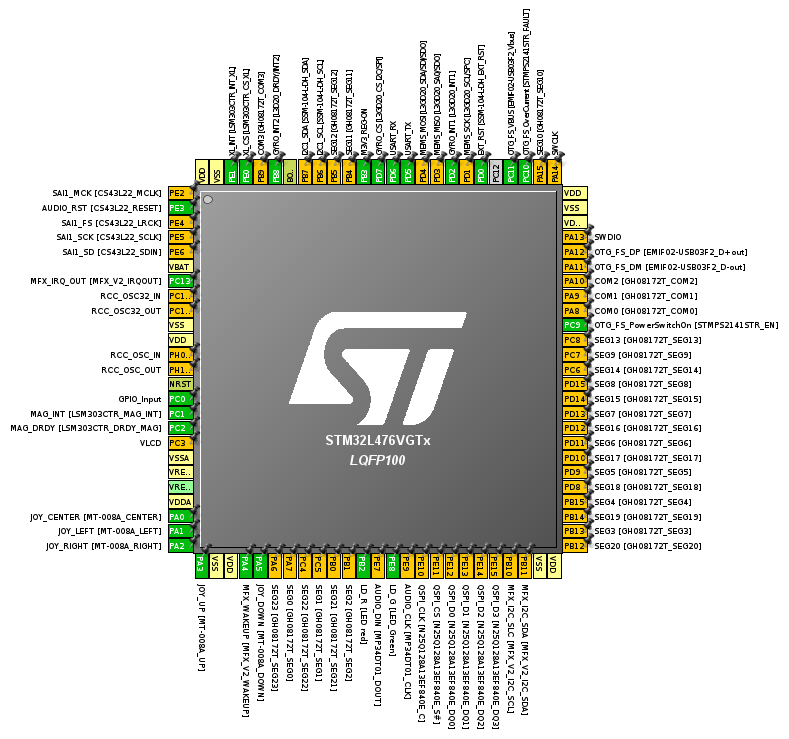
\includegraphics[width=0.85\textwidth]{../img/stm32disco.png}
    \caption{Procesor \textit{STM32L476VG}}
    \label{fig:stm32disco}
\end{figure}

Powyższy procesor może być taktowany zegarem o~częstotliwości równej aż
$80$~[$MHz$], co w~połączeniu z~wbudowanym koprocesorem zmiennoprzecinkowym
powinno pozwolić na symulowanie pracy układu chłodzenia w~czasie rzeczywistym.
W~tym momencie należy również zaznaczyć, iż podobnie jak rdzeń, koprocesor
zmiennoprzecinkowy operuje na słowach 32-bitowych, a~więc w~celu zapewnienia
sprzętowego wykonywania działań na liczbach zmiennoprzecikowych niezbędne było
korzystanie w~trakcie pisania kodu w~języku \textit{C++} z~danych typu
\textit{float}. Teoretycznie zapewniają one mniejszą dokładność, ale w~tym
przypadku pozwalają uniknąć programowego wykonywania operacji oraz zapewniają
dokładność wystarczającą do potrzeb, przez co użycie typu \textit{double} nie
było niezbędne.

Procesor ten przedstawiony został na rysunku~\ref{fig:stm32disco}. Na potrzeby
tego projektu wykorzystywane były jedynie wyprowadzenia PD5 oraz PD6 opisane
jako USART\_TX oraz USART\_RX.

\subsection{Algorytm rozwiązywania równań rożniczkowych}
\indent

Wykorzystana została metoda Rungego--Kutty czwartego rzędu, która jest jedną
z~najpopularniejszych metod numerycznych do iteracyjnego rozwiązywania równań
różniczkowych. Stosowana jest głównie z~powodu prostoty implementacji, dużej
szybkości oraz wysokiego rzędu.
Dysponując równaniem postaci:
\begin{equation*}
    \dot{x} = f\left( t, x \right)
\end{equation*}
w~którym znamy wartość $x(t_0) = x_0$, przyjmujemy dowolną wartość kroku
całkowania $dt$. Iteracyjny wzór metody RK4 jest następujący:
\begin{equation}
    x_{n+1} = x_n + \frac{k_1 + 2 \cdot k_2 + 2 \cdot k_3 + k4}{6}
    \label{equ:rk4}
\end{equation}
gdzie:
\begin{itemize}
    \item $k_1 = dt \cdot f\left( t_n, x_n \right)$,
    \item $k_2 = dt \cdot f\left( t_n + \frac{dt}{2}, x_n + \frac{k_1}{2}
    \right)$,
    \item $k_3 = dt \cdot f\left( t_n + \frac{dt}{2}, x_n + \frac{k_2}{2}
    \right)$,
    \item $k_4 = dt \cdot f\left( t_n + dt, x_n + k_3 \right)$.
\end{itemize}
Powyższy algorytm został zaimplementowany w~języku \textit{C++}.

\newpage
\subsection{Regulatory PID}
\indent

Do wyznaczania sterowań dla pompy wody oraz wentylatorów zostały stworzone
regulatory PID w~wersji dyskretnej opisane równaniem (w~wersji pozycyjnej):
\begin{equation}
    u_n = K_P \cdot e_n + K_I \cdot s_n + K_D \cdot d_n
    \label{equ:reg}
\end{equation}
gdzie:
\begin{itemize}
    \item $u_n$ --~sterowanie,
    \item $K_P$ --~wzmocnienie części proporcjonalnej,
    \item $K_I$ --~wzmocnienie części całkującej,
    \item $K_D$ --~wzmocnienie części różniczkującej,
    \item $e_n$ --~uchyb,
    \item $s_n$ --~suma uchybów dana zależnością:
        \begin{equation}
            s_n = s_{n - 1} + e_n
        \end{equation}
    \item $d_n$ --~różnica uchybów dana zależnością:
        \begin{equation}
            d_n = e_n - e_{n - 1}
        \end{equation}
\end{itemize}

Wartości poszczególnych wzmocnień nie były wyznaczane żadną specjalistyczną
metodą i~najczęściej wykorzystywaną konfiguracją była taka, w~której jedynie
część proporcjonalna posiadała wzmocnienie o~wartości równej $1$. Spowodowane to
było naciskiem na sprawdzenie poprawności samej implementacji modelu oraz
algorytmu rozwiązywania równań różniczkowych, a~także samego panelu
operatorskiego tworzonego na późniejszym etapie prac, aniżeli wyszukiwaniem
optymalnych nastaw względem wybranych wskaźników jakości sterowania.

\subsection{Wyjścia oraz wejścia systemu}
\indent

Stworzony model opisuje układ dwuwejściowy, w~którym możliwe jest sterowanie
pracą pompy wody oraz prędkością obrotową wentylatorów. W~odniesieniu do liczby
wyjść sytuacja jest nieco bardziej złożona, gdyż zależy głównie od wymagań
systemu. Podstawowym wyjściem jest temperatura procesora, która nie może
przekraczać wartości uznanych przez producenta za maksymalne bezpieczne, aby nie
doszło do uszkodzenia struktury krzemowej. Zwykle wynosi ona około
$100$~[$^\circ C$] i~po jej przekroczeniu następuje automatyczne obniżenie
częstotliwości taktowania rdzenia.

W~związku z~tym, w~tworzonym projekcie temperatura ta została wybrana jako
wyjście systemu i~to ona podlegała stabilizacji na zadanym poziomie w~trakcie
pracy układu. Na tej podstawie można stwierdzić, iż obiekt był typu MISO (ang.
Multiple Input Single Output).

W~rzeczywistych układach sytuacja jest bardziej skomplikowana, głównie z~powodu
wytrzymałości elementów systemu chłodzenia. Przykładowa pompa wody
\cite{EKWBpump} powinna pracować dla temperatur wody niższych niż $60$~[$^\circ
C$], w~związku z~czym wielkość ta również powinna podlegać stabilizacji na
poziomie odpowiednio niższym.

Ogromną zaletą rzeczywistych układów, które w~pewnym uproszczeniu zostały
opisane stworzonym modelem, jest jawna postać wszystkich zmiennych stanu, która
możliwa jest do uzyskania poprzez rozmieszczenie odpowiedniej liczby czujników
temperatury w~różnych miejscach pętli chłodzenia. Pozwala to uprościć
sterowanie, gdyż nie ma potrzeby tworzenia obserwatorów stanu, aby estymować
niejawne zmienne.

\subsection{Komunikacja z~komputerem}
\indent

Do komunikacji z~komputerem wykorzystany został port szeregowy. Peryferium
procesora pozwala wykorzystać jego pełną implementację zgodną ze standardem
\textit{RS-232}, lecz w~tym przypadku linie sterujące i~sygnalizujące były
zbędne, w~związku z~czym używano jedynie linii \textit{Rx} oraz \textit{Tx}. Ich
wyprowadzenie na płytce zostało oznaczone czerwonym okręgiem na
rysunku~\ref{fig:discovery}.

\begin{figure}[!ht]
    \centering
    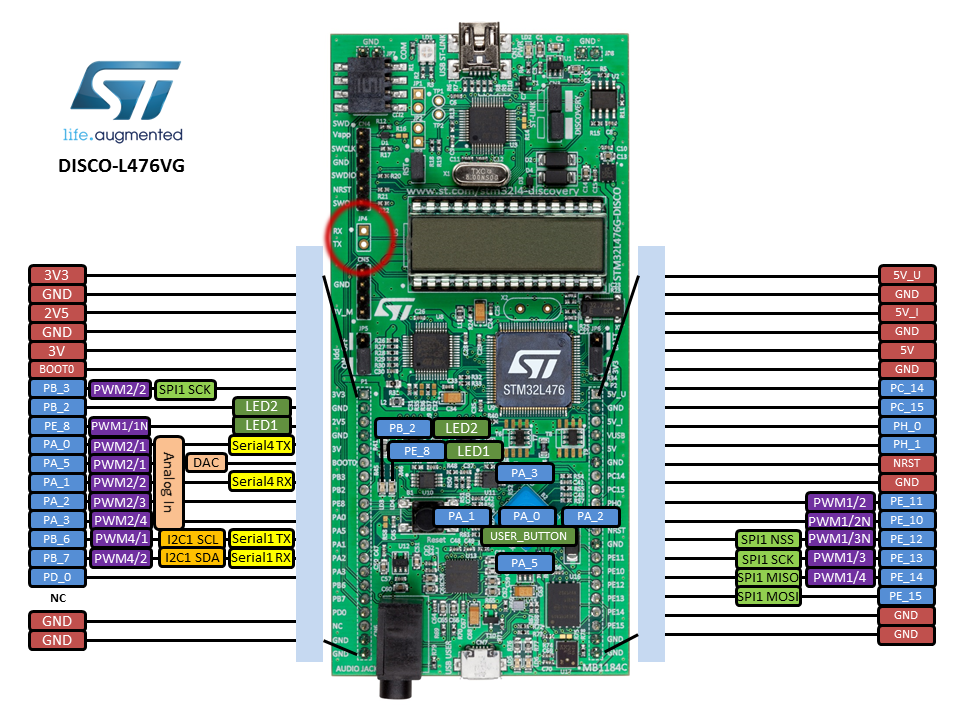
\includegraphics[width=\textwidth]{../img/discovery.png}
    \caption{Oznaczenie linii \textit{Rx} oraz \textit{Tx} na płytce
    \textit{32L476GDISCOVERY}}
    \label{fig:discovery}
\end{figure}

Jak już zostało jednak wspomniane we wcześniejszych rozdziałach, linie te są
jednocześnie podłączone do programatora, który pełni również rolę emulatora
portu szeregowego \textit{RS-232}. Dzięki temu, po podłączeniu płytki do
komputera bardzo szybko można zestawić połączenie z~układem. Podstawowym
zastosowaniem jest tutaj prototypowanie oraz przesyłanie pewnych informacji
kontrolnych, lecz ten projekt, zwłaszcza w~części poświęconej tworzeniu panelu
operatorskiego, miał za zadanie sprawdzić na ile taka komunikacja nadaje się do
zastosowań automatyki. Co ważne, w~początkowych etapach prac, które polegały na
stworzeniu oprogramowania na płytkę, komunikacja przebiegała bez najmniejszych
problemów i~była źródłem wielu informacji pozwalających znaleźć ewentualne
błędy.

Na potrzeby komunikacji przygotowane zostały odpowiednie struktury danych,
identyczne zarówno po stronie mikrokontrolera, jak i~komputera, które
przedstawione zostały na listingu~\ref{lst:commdata}. Dzięki temu, że zarówno
komputer, jak i~mikrokontroler posiadają ten sam system reprezentacji danych
wielobajtowych w~pamięci (LE, ang. Little Endian), nie było potrzeby dokonywania
żadnych pośrednich konwersji w~trakcie wymiany informacji pomiędzy nimi.

\begin{figure}[!ht]
    \lstinputlisting[caption=Struktury
    danych wykorzystywane
    w~komunikacji,label=lst:commdata]{../../dev/WCSim/CommunicationData.h}
\end{figure}
Pierwsza z~nich, \textit{OutData}, zawiera dane dotyczące stanu symulacji
działania układu chłodzenia wysyłane z~mikrokontrolera do komputera:
\begin{itemize}
    \item \textit{mTime} --~aktualny czas działania układu w~sekundach,
    \item \textit{mState} --~tablica zawierająca wszystkie wartości zmiennych
    stanu, zgodnie z~układem równań \eqref{equ:model}.
\end{itemize}

Druga, \textit{PID}, jest strukturą pomocniczą i~zawiera pola z~nastawami
regulatora odpowiadające tym ze wzoru \eqref{equ:reg}:
\begin{itemize}
    \item \textit{mP} --~wartość wzmocnienia części proporcjonalnej,
    \item \textit{mI} --~wartość wzmocnienia części całkującej,
    \item \textit{mD} --~wartość wzmocnienia części różniczkującej.
\end{itemize}

Ostatnia, \textit{InData}, zawiera informacje sterujące przesyłane z~komputera
do mikronkontrolera, które służą do zmiany nastaw regulatorów oraz są
wykorzystywane w~trakcie rozwiązywania układu równań \eqref{equ:model}:
\begin{itemize}
    \item \textit{mPID1} --~nastawy regulatora pompy wody,
    \item \textit{mPID2} --~nastawy regulatora prędkości obrotowej wentylatorów,
    \item \textit{mSetPoint} --~wartość zadana temperatury procesora,
    \item \textit{mPower} --~moc wydzielana w~rdzeniu procesora,
    \item \textit{mTo} --~wartość temperatury otoczenia radiatora.
\end{itemize}

%     \include{algorytm}
%     \include{problem}
%     \include{eksperymenty}
%     \section{Wnioski}
\indent

Cel opisanego we wcześniejszych rozdziałach projektu, którym było stworzenie
symulatora układu chłodzenia cieczą procesora komputera oraz stworzenie panelu
operatorskiego z~wykorzystaniem biblioteki \textit{Qt} w~języku \textit{C++}
może być z~pewnością uznany za osiągnięty.

Praca nad tym projektem pozwoliła spojrzeć w~zupełnie inny sposób na tworzenie
oprogramowania typu SCADA, gdyż to na autorach spoczywała odpowiedzialność za
wprowadzenie odpowiedniej funkcjonalności do programu oraz zapewnienie
skuteczności jego działania. W~trakcie prac udało się zauważyć zarówno zalety,
jak i~pewne wady oprogramowania specjalistycznego. Do tych pierwszych zaliczały
się na pewno:
\begin{itemize}
    \item możliwość utworzenia panelu operatorskiego dla dowolnego procesu,
    \item kompatybilność z~dużą ilością sprzętu dostępnego na rynku,
    \item łatwość zmiany konfiguracji utworzonego programu.
\end{itemize}
Jednak część z~tych zalet może bardzo łatwo obrócić się w~wady, przynajmniej dla
użytkownika, który szuka prostszych rozwiązań na potrzeby kontrolowania
niewielkiego i~nieskomplikowanego procesu technologicznego. Podobne odczucia
posiadali autorzy, gdy odbywali pierwsze zajęcia z~wykorzystaniem programu
\textit{zenon}, gdy mnogość dostępnych opcji utrudniała wielokrotnie
odnalezienie tych właściwych, w~danym momencie wymaganych.

O~ile realizowany projekt był pewnego rodzaju eksperymentem mającym sprawdzić,
jakie nakłady pracy są niezbędne do stworzenia panelu operatorskiego dla
zadanego procesu technologicznego oraz ile problemów może to sprawić, o~tyle
należy w~tym miejscu przyznać, że dzięki znajomości narzędzi, które były
wykorzystywane w~trakcie pracy udało się osiągnąć efekt bez większych problemów
po drodze.

Podsumowując, oprogramowanie typu SCADA stworzone przez wyspecjalizowane firmy
jest potężnym narzędziem pozwalającym na przygotowanie paneli operatorskich oraz
innych narzędzi niezbędnych do prawidłowego zarządzania procesami
technologicznymi. Mimo wszystko, autorzy uważają, że w~wielu przypadkach,
zarówno hobbystycznych, jak i~w~odniesieniu do prostych procesów realizowanych
w~mniejszych lub większych zakładach pracy, dowiedzenie możliwości utworzenia
oprogramowania przygotowanego do pracy w~specyficznych i~z~góry znanych
warunkach jest niewątpliwie bardzo dobrym rezultatem wykonanych prac.

%     \include{listings}
    \begin{thebibliography}{9}

    \bibitem{EKWBsite}
        \textit{EKWB --~Premium Liquid Cooling solutions},\\
        \verb+https://www.ekwb.com+,\\
        dostęp: 17 stycznia 2017
        
    \bibitem{EKWBpump}
        \textit{EK-D5 PWM G2 Motor},
        \textit{EK Webshop},\\
        \verb+https://www.ekwb.com/shop/ek-d5-pwm-g2-motor-12v-dc-pwm-pump-motor+,\\
        dostęp: 17 stycznia 2017
        
    \bibitem{EKWBfan}
        \textit{EK-Furious Vardar FF5-120},
        \textit{EK Webshop},\\
        \verb+https://www.ekwb.com/shop/ek-furious-vardar-ff5-120-3000rpm+,\\
        dostęp: 17 stycznia 2017
    
    \bibitem{EKWBradiator}
        \textit{EK-CoolStream PE 480},
        \textit{EK Webshop},\\
        \verb+https://www.ekwb.com/shop/ek-coolstream-pe-480-quad+,\\
        dostęp: 17 stycznia 2017
        
    \bibitem{ThermalResistance}
        \textit{Rezystancja termiczna},
        \textit{Wikipedia, Wolna encyklopedia},\\
        \verb+https://pl.wikipedia.org/wiki/Rezystancja_termiczna+,\\
        dostęp: 17 stycznia 2017
        
    \bibitem{Inteli7}
        \textit{Intel Core i7-5960X Processor Extereme Edition},
        \textit{Intel},\\
        \verb+http://ark.intel.com/pl/products/82930/Intel-Core-i7-5960X-Processor+\\
        \verb+-Extreme-Edition-20M-Cache-up-to-3_50-GHz+,\\
        dostęp: 17 stycznia 2017
        
    \bibitem{CHT}
        \textit{Convective Heat Transfer},
        \textit{The Engineering ToolBox},\\
        \verb+http://www.engineeringtoolbox.com/convective-heat-transfer-d_430.html+,\\
        dostęp: 17 stycznia 2017
        
    \bibitem{STM32}
        \textit{32l476GDISCOVERY --~Discovery kit with STM32L476VG MCU},
        \textit{STMicroelectronics},\\
        \verb+http://www.st.com/en/evaluation-tools/32l476gdiscovery.html+,\\
        dostęp: 17 stycznia 2017

\end{thebibliography}
    
\end{document}